\section{Experiments and Results}

\subsection{Design Challenges}
\begin{enumroman}
  \item I was not sure if this is a standard change,
    but \lstinline{scipy.signal.gaussian} seems to have been
    migrated to \lstinline{scipy.signal.windows.gaussian}
    in Python 3.11 (see \href{https://docs.scipy.org/doc/scipy/reference/generated/scipy.signal.windows.gaussian.html}{here}).
  \item I spent a few hours debugging my hough transform,
    only to realize that writing into and reading from
    an array concurrently was resulting in
    inaccuracies.
    Fixing this issue made everything work.
  \item I also had a bug in my gaussian kernel
     --- I was resizing the kernel but not normalizing it
    back to sum up to $1$, which resulted in
    a lot of spurious and inaccurate lines.
    This was a definitive fix, but debugging it took a while.
\end{enumroman}

\subsection{Experiments}

I played around with some of the parameters to see how the results
are affected.

\begin{enumroman}
  \item \textbf{gaussian kernel variance ($\sigma$):}
    Increasing the value of $\sigma$ improves the image detection up to a point,
    then flattens out the line once $\sigma$ goes beyond the optimal value.
    I found the best results with $\sigma = 2$ to work well for most of my images,
    although $\sigma = 3$ seemed to work better on one image.
  \item \textbf{threshold:}
    Raising the threshold prunes erratic lines in the image,
    but if the threshold is too high, accurate lines are pruned too
    (see image).
    I found the best results with a threshold of $0.3$.

    \begin{figure}[h]
      \centering
      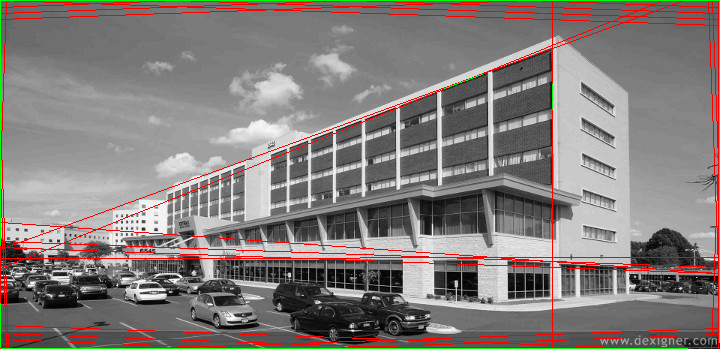
\includegraphics[width=0.8\textwidth]{09-threshold-0.5.png}
      \caption{Threshold = $0.5$}
      \label{fig:threshold}
    \end{figure}
  \item \textbf{theta resolution:}
    Increasing the resolution of $\theta$ increases the accuracy
    of the lines found in the image, but it also increases the
    computation time. I found the best results with a resolution
    of $\frac{\pi}{180}$, but I settled on $\frac{pi}{90}$
    because the latter takes significantly less time to compute
    and the difference in accuracy is not too extreme.

  \item \textbf{rho resolution:}
    I also found that increasing the resolution of $\rho$
    increases the accuracy of the lines found
    also increases the computation time.

  \item \textbf{number of lines:}
    This yielded varying results depending on the image.
    While a specific number of lines would cause the algorithm
    to ignore correct lines in one image, the same might cause less
    accurate lines to be admitted in another image.
    This clearly needs to be tuned specific to every image
\end{enumroman}

\newpage
\subsection{Results}

These were the results I got for image 01.

\begin{figure}[h]
  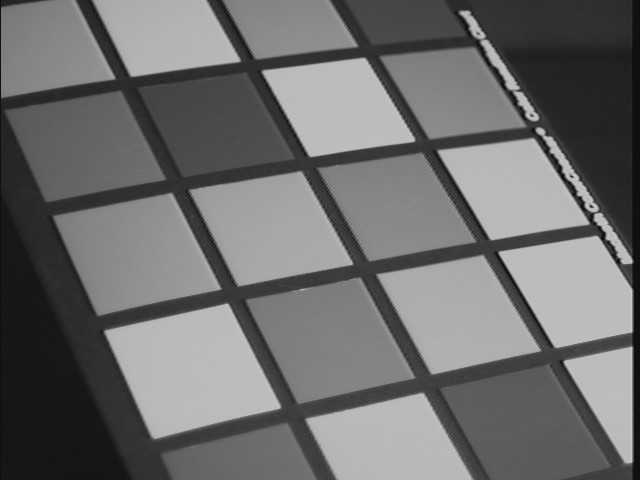
\includegraphics[width=0.5\textwidth]{img01.jpg}
  \caption{Original image}
  \label{fig:original}
\end{figure}


\begin{figure}[h!]
  \includegraphics*[width=0.5\textwidth]{01-edge.png}
  \caption{Edge Detection}
  \label{fig:edge}
\end{figure}

\begin{figure}[h!]
  \includegraphics*[width=0.5\textwidth]{01-threshold.png}
  \caption{Thresholding}
  \label{fig:threshold}
\end{figure}

\begin{figure}[h]
  \includegraphics*[height=0.5\textwidth]{01-hough.png}
  \caption{Hough Transform}
  \label{fig:hough}
\end{figure}

\begin{figure}[h]
  \includegraphics*[width=0.5\textwidth]{01-lines.png}
  \caption{Line Detection}
  \label{fig:lines}
\end{figure}
